%% fig_diagonalbudget.tex   (generated by make_round32.py; do not edit by hand)
%% The 525 diagonal classes of degree two at n = 3: what the cup products remove, what the fourfold products can remove for each gap t_2 - t_1, and the 57 the criterion asks for (prop:cupkernel, thm:esixdiagonal); beside it the components of the graphs Gamma_tau on the 32 pieces L_zeta.
\documentclass[tikz,border=8pt]{standalone}
\usepackage{amsmath,amssymb}
\usetikzlibrary{arrows.meta,calc,decorations.pathreplacing}
%% palette.tex -- shared colour definitions for the figures
\definecolor{PInk}{RGB}{26,32,44}
\definecolor{PBlue}{RGB}{37,82,139}
\definecolor{PTeal}{RGB}{23,127,125}
\definecolor{POchre}{RGB}{193,138,44}
\definecolor{PClay}{RGB}{178,74,58}
\definecolor{PSlate}{RGB}{108,122,137}
\definecolor{PViolet}{RGB}{110,86,150}
\definecolor{WBlue}{RGB}{223,234,246}
\definecolor{WTeal}{RGB}{220,238,236}
\definecolor{WOchre}{RGB}{250,240,218}
\definecolor{WClay}{RGB}{247,229,224}
\definecolor{WSlate}{RGB}{238,241,244}
\definecolor{PMag}{RGB}{158,58,110}
\definecolor{PGrass}{RGB}{62,124,66}
\definecolor{PAmber}{RGB}{214,112,38}
\definecolor{PIndigo}{RGB}{58,64,140}
\definecolor{PRule}{RGB}{176,186,197}

%% shared macros so the standalone figures match the paper
\providecommand{\QQ}{\mathbb{Q}}
\providecommand{\ZZ}{\mathbb{Z}}
\providecommand{\RR}{\mathbb{R}}
\providecommand{\CC}{\mathbb{C}}
\providecommand{\PP}{\mathbb{P}}
\providecommand{\Kx}{K^{\times}}
\providecommand{\HW}{W}
\providecommand{\Nm}{\mathrm{N}}
\providecommand{\Hdg}{\mathrm{Hdg}}
\providecommand{\NS}{\mathrm{NS}}
\providecommand{\cA}{\mathcal{A}}
\providecommand{\cD}{\mathcal{D}}
\providecommand{\cF}{\mathcal{F}}
\providecommand{\cP}{\mathcal{P}}
\providecommand{\cO}{\mathcal{O}}
\providecommand{\cQ}{\mathcal{Q}}
\providecommand{\bbar}[1]{\overline{#1}}
\providecommand{\ch}{\operatorname{ch}}
\providecommand{\End}{\mathrm{End}}
\providecommand{\Ext}{\operatorname{Ext}}
\providecommand{\Supp}{\operatorname{Supp}}

\begin{document}
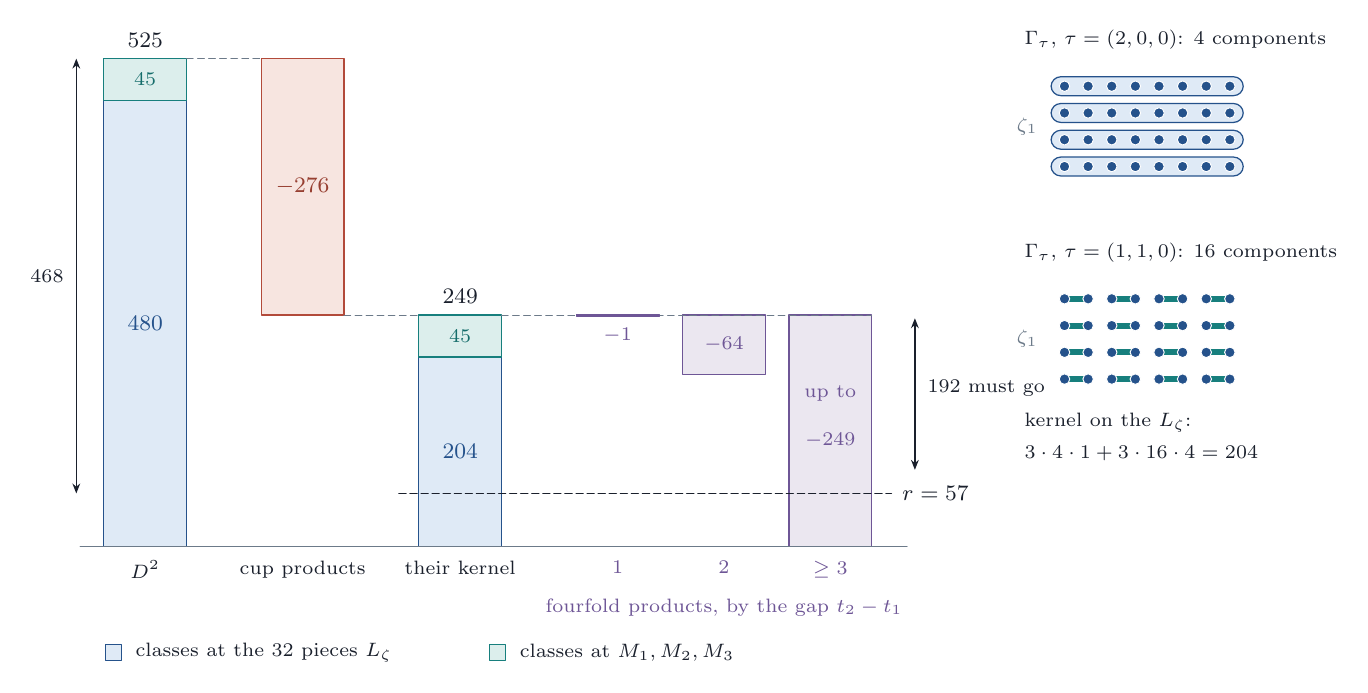
\begin{tikzpicture}[x=1cm,y=1cm,line join=round,line cap=round,
  font=\small,text=PInk,lbl/.style={inner sep=1pt}]
  \path[fill=WBlue,draw=PBlue,line width=0.45pt] (0.0000,0.0000) rectangle (1.0500,5.6640);
  \path[fill=WTeal,draw=PTeal,line width=0.45pt] (0.0000,5.6640) rectangle (1.0500,6.1950);
  \path[fill=WClay,draw=PClay,line width=0.45pt] (2.0000,2.9382) rectangle (3.0500,6.1950);
  \path[fill=WBlue,draw=PBlue,line width=0.45pt] (4.0000,0.0000) rectangle (5.0500,2.4072);
  \path[fill=WTeal,draw=PTeal,line width=0.45pt] (4.0000,2.4072) rectangle (5.0500,2.9382);
  \path[fill=PViolet!14!white,draw=PViolet,line width=0.45pt] (7.3500,2.1830) rectangle (8.4000,2.9382);
  \path[fill=PViolet!14!white,draw=PViolet,line width=0.45pt] (8.7000,0.0000) rectangle (9.7500,2.9382);
  \draw[PSlate,line width=0.5pt] (-0.3000,0.0000) -- (10.2000,0.0000);
  \draw[PSlate,line width=0.4pt,dash pattern=on 2.4pt off 1.6pt] (1.0500,6.1950) -- (2.0000,6.1950);
  \draw[PSlate,line width=0.4pt,dash pattern=on 2.4pt off 1.6pt] (3.0500,2.9382) -- (4.0000,2.9382);
  \draw[PSlate,line width=0.4pt,dash pattern=on 2.4pt off 1.6pt] (5.0500,2.9382) -- (9.7500,2.9382);
  \path[fill=PViolet,draw=PViolet,line width=0.30pt] (6.0000,2.9262) rectangle (7.0500,2.9502);
  \draw[PInk,line width=0.7pt,dash pattern=on 2.4pt off 1.6pt] (3.7500,0.6726) -- (10.0000,0.6726);
  \draw[PInk,line width=0.5pt,{Stealth[length=3.6pt,width=2.8pt]}-{Stealth[length=3.6pt,width=2.8pt]}] (10.3000,0.9726) -- (10.3000,2.8982);
  \draw[PInk,line width=0.5pt,{Stealth[length=3.6pt,width=2.8pt]}-{Stealth[length=3.6pt,width=2.8pt]}] (-0.3500,0.6726) -- (-0.3500,6.1950);
  \path[fill=WBlue,draw=PBlue,line width=0.45pt] (0.0200,-1.4500) rectangle (0.2200,-1.2500);
  \path[fill=WTeal,draw=PTeal,line width=0.45pt] (4.9000,-1.4500) rectangle (5.1000,-1.2500);
  \path[fill=WBlue,draw=PBlue,line width=0.45pt,rounded corners=3.5pt] (12.0300,5.7250) rectangle (14.4700,5.9650);
  \path[fill=PBlue,draw=white,line width=0.35pt] (12.2000,5.8450) circle (1.90pt);
  \path[fill=PBlue,draw=white,line width=0.35pt] (12.5000,5.8450) circle (1.90pt);
  \path[fill=PBlue,draw=white,line width=0.35pt] (12.8000,5.8450) circle (1.90pt);
  \path[fill=PBlue,draw=white,line width=0.35pt] (13.1000,5.8450) circle (1.90pt);
  \path[fill=PBlue,draw=white,line width=0.35pt] (13.4000,5.8450) circle (1.90pt);
  \path[fill=PBlue,draw=white,line width=0.35pt] (13.7000,5.8450) circle (1.90pt);
  \path[fill=PBlue,draw=white,line width=0.35pt] (14.0000,5.8450) circle (1.90pt);
  \path[fill=PBlue,draw=white,line width=0.35pt] (14.3000,5.8450) circle (1.90pt);
  \path[fill=WBlue,draw=PBlue,line width=0.45pt,rounded corners=3.5pt] (12.0300,5.3850) rectangle (14.4700,5.6250);
  \path[fill=PBlue,draw=white,line width=0.35pt] (12.2000,5.5050) circle (1.90pt);
  \path[fill=PBlue,draw=white,line width=0.35pt] (12.5000,5.5050) circle (1.90pt);
  \path[fill=PBlue,draw=white,line width=0.35pt] (12.8000,5.5050) circle (1.90pt);
  \path[fill=PBlue,draw=white,line width=0.35pt] (13.1000,5.5050) circle (1.90pt);
  \path[fill=PBlue,draw=white,line width=0.35pt] (13.4000,5.5050) circle (1.90pt);
  \path[fill=PBlue,draw=white,line width=0.35pt] (13.7000,5.5050) circle (1.90pt);
  \path[fill=PBlue,draw=white,line width=0.35pt] (14.0000,5.5050) circle (1.90pt);
  \path[fill=PBlue,draw=white,line width=0.35pt] (14.3000,5.5050) circle (1.90pt);
  \path[fill=WBlue,draw=PBlue,line width=0.45pt,rounded corners=3.5pt] (12.0300,5.0450) rectangle (14.4700,5.2850);
  \path[fill=PBlue,draw=white,line width=0.35pt] (12.2000,5.1650) circle (1.90pt);
  \path[fill=PBlue,draw=white,line width=0.35pt] (12.5000,5.1650) circle (1.90pt);
  \path[fill=PBlue,draw=white,line width=0.35pt] (12.8000,5.1650) circle (1.90pt);
  \path[fill=PBlue,draw=white,line width=0.35pt] (13.1000,5.1650) circle (1.90pt);
  \path[fill=PBlue,draw=white,line width=0.35pt] (13.4000,5.1650) circle (1.90pt);
  \path[fill=PBlue,draw=white,line width=0.35pt] (13.7000,5.1650) circle (1.90pt);
  \path[fill=PBlue,draw=white,line width=0.35pt] (14.0000,5.1650) circle (1.90pt);
  \path[fill=PBlue,draw=white,line width=0.35pt] (14.3000,5.1650) circle (1.90pt);
  \path[fill=WBlue,draw=PBlue,line width=0.45pt,rounded corners=3.5pt] (12.0300,4.7050) rectangle (14.4700,4.9450);
  \path[fill=PBlue,draw=white,line width=0.35pt] (12.2000,4.8250) circle (1.90pt);
  \path[fill=PBlue,draw=white,line width=0.35pt] (12.5000,4.8250) circle (1.90pt);
  \path[fill=PBlue,draw=white,line width=0.35pt] (12.8000,4.8250) circle (1.90pt);
  \path[fill=PBlue,draw=white,line width=0.35pt] (13.1000,4.8250) circle (1.90pt);
  \path[fill=PBlue,draw=white,line width=0.35pt] (13.4000,4.8250) circle (1.90pt);
  \path[fill=PBlue,draw=white,line width=0.35pt] (13.7000,4.8250) circle (1.90pt);
  \path[fill=PBlue,draw=white,line width=0.35pt] (14.0000,4.8250) circle (1.90pt);
  \path[fill=PBlue,draw=white,line width=0.35pt] (14.3000,4.8250) circle (1.90pt);
  \draw[PTeal,line width=2.2pt] (12.2000,3.1450) -- (12.5000,3.1450);
  \path[fill=PBlue,draw=white,line width=0.35pt] (12.2000,3.1450) circle (1.90pt);
  \path[fill=PBlue,draw=white,line width=0.35pt] (12.5000,3.1450) circle (1.90pt);
  \draw[PTeal,line width=2.2pt] (12.8000,3.1450) -- (13.1000,3.1450);
  \path[fill=PBlue,draw=white,line width=0.35pt] (12.8000,3.1450) circle (1.90pt);
  \path[fill=PBlue,draw=white,line width=0.35pt] (13.1000,3.1450) circle (1.90pt);
  \draw[PTeal,line width=2.2pt] (13.4000,3.1450) -- (13.7000,3.1450);
  \path[fill=PBlue,draw=white,line width=0.35pt] (13.4000,3.1450) circle (1.90pt);
  \path[fill=PBlue,draw=white,line width=0.35pt] (13.7000,3.1450) circle (1.90pt);
  \draw[PTeal,line width=2.2pt] (14.0000,3.1450) -- (14.3000,3.1450);
  \path[fill=PBlue,draw=white,line width=0.35pt] (14.0000,3.1450) circle (1.90pt);
  \path[fill=PBlue,draw=white,line width=0.35pt] (14.3000,3.1450) circle (1.90pt);
  \draw[PTeal,line width=2.2pt] (12.2000,2.8050) -- (12.5000,2.8050);
  \path[fill=PBlue,draw=white,line width=0.35pt] (12.2000,2.8050) circle (1.90pt);
  \path[fill=PBlue,draw=white,line width=0.35pt] (12.5000,2.8050) circle (1.90pt);
  \draw[PTeal,line width=2.2pt] (12.8000,2.8050) -- (13.1000,2.8050);
  \path[fill=PBlue,draw=white,line width=0.35pt] (12.8000,2.8050) circle (1.90pt);
  \path[fill=PBlue,draw=white,line width=0.35pt] (13.1000,2.8050) circle (1.90pt);
  \draw[PTeal,line width=2.2pt] (13.4000,2.8050) -- (13.7000,2.8050);
  \path[fill=PBlue,draw=white,line width=0.35pt] (13.4000,2.8050) circle (1.90pt);
  \path[fill=PBlue,draw=white,line width=0.35pt] (13.7000,2.8050) circle (1.90pt);
  \draw[PTeal,line width=2.2pt] (14.0000,2.8050) -- (14.3000,2.8050);
  \path[fill=PBlue,draw=white,line width=0.35pt] (14.0000,2.8050) circle (1.90pt);
  \path[fill=PBlue,draw=white,line width=0.35pt] (14.3000,2.8050) circle (1.90pt);
  \draw[PTeal,line width=2.2pt] (12.2000,2.4650) -- (12.5000,2.4650);
  \path[fill=PBlue,draw=white,line width=0.35pt] (12.2000,2.4650) circle (1.90pt);
  \path[fill=PBlue,draw=white,line width=0.35pt] (12.5000,2.4650) circle (1.90pt);
  \draw[PTeal,line width=2.2pt] (12.8000,2.4650) -- (13.1000,2.4650);
  \path[fill=PBlue,draw=white,line width=0.35pt] (12.8000,2.4650) circle (1.90pt);
  \path[fill=PBlue,draw=white,line width=0.35pt] (13.1000,2.4650) circle (1.90pt);
  \draw[PTeal,line width=2.2pt] (13.4000,2.4650) -- (13.7000,2.4650);
  \path[fill=PBlue,draw=white,line width=0.35pt] (13.4000,2.4650) circle (1.90pt);
  \path[fill=PBlue,draw=white,line width=0.35pt] (13.7000,2.4650) circle (1.90pt);
  \draw[PTeal,line width=2.2pt] (14.0000,2.4650) -- (14.3000,2.4650);
  \path[fill=PBlue,draw=white,line width=0.35pt] (14.0000,2.4650) circle (1.90pt);
  \path[fill=PBlue,draw=white,line width=0.35pt] (14.3000,2.4650) circle (1.90pt);
  \draw[PTeal,line width=2.2pt] (12.2000,2.1250) -- (12.5000,2.1250);
  \path[fill=PBlue,draw=white,line width=0.35pt] (12.2000,2.1250) circle (1.90pt);
  \path[fill=PBlue,draw=white,line width=0.35pt] (12.5000,2.1250) circle (1.90pt);
  \draw[PTeal,line width=2.2pt] (12.8000,2.1250) -- (13.1000,2.1250);
  \path[fill=PBlue,draw=white,line width=0.35pt] (12.8000,2.1250) circle (1.90pt);
  \path[fill=PBlue,draw=white,line width=0.35pt] (13.1000,2.1250) circle (1.90pt);
  \draw[PTeal,line width=2.2pt] (13.4000,2.1250) -- (13.7000,2.1250);
  \path[fill=PBlue,draw=white,line width=0.35pt] (13.4000,2.1250) circle (1.90pt);
  \path[fill=PBlue,draw=white,line width=0.35pt] (13.7000,2.1250) circle (1.90pt);
  \draw[PTeal,line width=2.2pt] (14.0000,2.1250) -- (14.3000,2.1250);
  \path[fill=PBlue,draw=white,line width=0.35pt] (14.0000,2.1250) circle (1.90pt);
  \path[fill=PBlue,draw=white,line width=0.35pt] (14.3000,2.1250) circle (1.90pt);
  \node[lbl,text=PBlue,font=\footnotesize] at (0.5250,2.8320) {$480$};
  \node[lbl,text=PTeal!85!black,font=\scriptsize] at (0.5250,5.9295) {$45$};
  \node[lbl,anchor=south,text=PInk,font=\footnotesize] at (0.5250,6.2950) {$525$};
  \node[lbl,text=PClay!85!black,font=\footnotesize] at (2.5250,4.5666) {$-276$};
  \node[lbl,text=PBlue,font=\footnotesize] at (4.5250,1.2036) {$204$};
  \node[lbl,text=PTeal!85!black,font=\scriptsize] at (4.5250,2.6727) {$45$};
  \node[lbl,anchor=south,text=PInk,font=\footnotesize] at (4.5250,3.0382) {$249$};
  \node[lbl,anchor=north,text=PViolet,font=\scriptsize] at (6.5250,2.8182) {$-1$};
  \node[lbl,text=PViolet,font=\scriptsize] at (7.8750,2.5606) {$-64$};
  \node[lbl,text=PViolet,font=\scriptsize] at (9.2250,1.9411) {up to};
  \node[lbl,text=PViolet,font=\scriptsize] at (9.2250,1.3511) {$-249$};
  \node[lbl,anchor=west,text=PInk,font=\footnotesize] at (10.1000,0.6726) {$r=57$};
  \node[lbl,anchor=west,text=PInk,font=\scriptsize] at (10.4200,2.0054) {$192$ must go};
  \node[lbl,anchor=east,text=PInk,font=\scriptsize] at (-0.4700,3.4338) {$468$};
  \node[lbl,anchor=north,text=PInk,font=\scriptsize] at (0.5250,-0.1400) {$D^{2}$};
  \node[lbl,anchor=north,text=PInk,font=\scriptsize] at (2.5250,-0.1400) {cup products};
  \node[lbl,anchor=north,text=PInk,font=\scriptsize] at (4.5250,-0.1400) {their kernel};
  \node[lbl,anchor=north,text=PViolet,font=\scriptsize] at (6.5250,-0.1400) {$1$};
  \node[lbl,anchor=north,text=PViolet,font=\scriptsize] at (7.8750,-0.1400) {$2$};
  \node[lbl,anchor=north,text=PViolet,font=\scriptsize] at (9.2250,-0.1400) {$\ge3$};
  \node[lbl,anchor=north,text=PViolet,font=\scriptsize] at (7.8750,-0.6200) {fourfold products, by the gap $t_{2}-t_{1}$};
  \node[lbl,anchor=west,text=PInk,font=\scriptsize] at (0.3600,-1.3500) {classes at the $32$ pieces $L_{\zeta}$};
  \node[lbl,anchor=west,text=PInk,font=\scriptsize] at (5.2400,-1.3500) {classes at $M_{1},M_{2},M_{3}$};
  \node[lbl,anchor=west,text=PInk,font=\scriptsize] at (11.6500,6.4302) {$\Gamma_{\tau}$, $\tau=(2,0,0)$: $4$ components};
  \node[lbl,anchor=east,text=PSlate,font=\scriptsize] at (11.9000,5.3350) {$\zeta_{1}$};
  \node[lbl,anchor=west,text=PInk,font=\scriptsize] at (11.6500,3.7302) {$\Gamma_{\tau}$, $\tau=(1,1,0)$: $16$ components};
  \node[lbl,anchor=east,text=PSlate,font=\scriptsize] at (11.9000,2.6350) {$\zeta_{1}$};
  \node[lbl,anchor=west,text=PInk,font=\scriptsize] at (11.6500,1.5717) {kernel on the $L_{\zeta}$:};
  \node[lbl,anchor=west,text=PInk,font=\scriptsize] at (11.6500,1.1789) {$3\cdot4\cdot1+3\cdot16\cdot4=204$};
\end{tikzpicture}
\end{document}
